\documentclass[border=4pt]{standalone}
% Preámbulo común de las figuras. Cada figura es un documento standalone
% que se compila a SVG con scripts/build_figures.sh
\usepackage[utf8]{inputenc}
\usepackage{amsmath}
\usepackage{tikz}
\usepackage[american, siunitx]{circuitikz}
\usetikzlibrary{arrows.meta,calc,decorations.pathmorphing,patterns}
\tikzset{
  >={Stealth[length=2.2mm]},
  eje/.style={->, thin},
  hilo/.style={thick},
}
% Paleta común: tonos medios legibles sobre fondo claro
\definecolor{azul}{RGB}{31,94,168}
\definecolor{rojo}{RGB}{192,57,43}
\definecolor{verde}{RGB}{39,128,73}
\definecolor{naranja}{RGB}{211,120,30}
\definecolor{morado}{RGB}{125,60,152}

\begin{document}
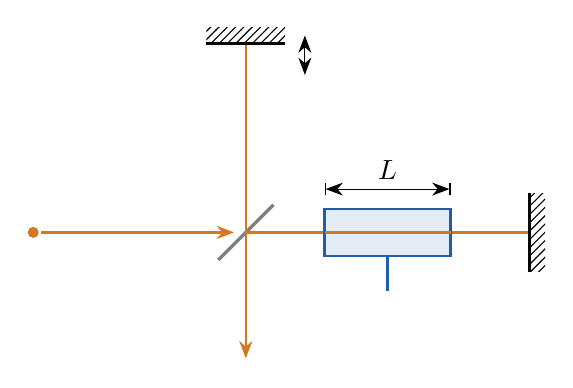
\begin{tikzpicture}[scale=1.0]
  \draw[naranja, thick, ->] (-2.6,0) -- (-0.15,0);
  \fill[naranja] (-2.7,0) circle (2pt);
  % divisor de haz
  \draw[very thick, gray] (-0.35,-0.35) -- (0.35,0.35);
  % brazo vertical hacia el espejo móvil
  \draw[naranja, thick] (0,0) -- (0,2.4);
  \fill[pattern=north east lines] (-0.5,2.4) rectangle (0.5,2.6);
  \draw[very thick] (-0.5,2.4) -- (0.5,2.4);
  \draw[<->] (0.75,2.5) -- (0.75,2.0);
  % brazo horizontal con la celda
  \draw[naranja, thick] (0,0) -- (3.6,0);
  \filldraw[draw=azul, fill=azul!12, thick] (1.0,-0.3) rectangle (2.6,0.3);
  \draw[naranja, thick] (1.0,0) -- (2.6,0);
  \draw[thick, azul] (1.8,-0.3) -- (1.8,-0.75);
  \draw[|<->|] (1.0,0.55) -- node[above]{$L$} (2.6,0.55);
  \fill[pattern=north east lines] (3.6,-0.5) rectangle (3.8,0.5);
  \draw[very thick] (3.6,-0.5) -- (3.6,0.5);
  % hacia el observador
  \draw[naranja, thick, ->] (0,0) -- (0,-1.6);
\end{tikzpicture}
\end{document}
